\section{Cherenkov-Detektoren}

\chapterauthor{Rune Dominik, 26.10.2018}

\subsection{Geschichte}
Tatsächlich hat bereits Marie Curie blaues Licht gesehen, was heute als Cherenkovlicht erklärt werden kann.

\subsection{Theorie}
Der Cherenkoveffekt tritt auf, wenn geladene Teilchen mit Überlichtgeschwindigkeit durch ein Medium propagieren. Es wird hierdurch ein Cherekovlichtkegel abgegeben, siehe Abbildung \ref{fig:aufbau}.

\begin{figure}[H]
  \centering
  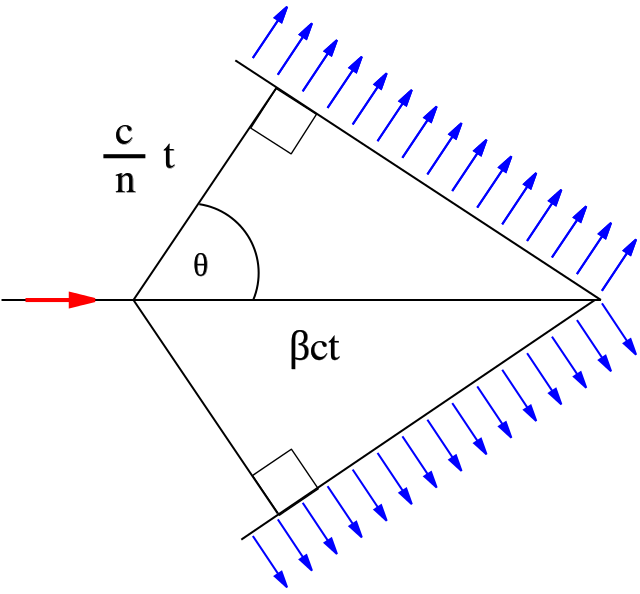
\includegraphics[height=6.0cm]{content/Cherenkov.png}
  \caption{Theoretische Erklärung des Cherenkoveffektes.}
  \label{fig:aufbau}
\end{figure}

\subsection{Aufbau}
Es gibt verschiedene Bauweisen für solche Teleskope. Insbesondere die HESE ist eine sehr moderne Bauweise.

Test~\cite{Gil:02}


